\section{Introduction}
\label{sect:introduction}

Supersymmetry  (SUSY) \cite{Golfand:1971iw,Wess:1973kz,Wess:1974tw,Fayet1,Fayet2} is one of the most promising extensions of the 
standard model (SM) of elementary particles.  It leads to the unification of gauge couplings at
high energy, it mitigates the problem of quadratic divergences in quantum corrections to the
mass of the Higgs boson, and, in its R-parity-conserving realization, provides a dark matter candidate.
A key prediction of SUSY is the existence of new particles with the same properties as SM particles but
differing in spin by half a unit (``sparticles'').
%
%which solves the 
%quadratic divergences in the corrections to the mass of the Higgs boson from the fermions by introducing the new
%bosons with proper couplings. The newly defined particles can fill the scales between the electroweak scale and 
%the upper limit of the validity of SM and solve the  hierarchy problems, simultaneously. 
%It introduces a new symmetry between the bosons and fermions and 
%for every particle a sparticle is defined which is exactly the same, but differs in spin by 1/2. 
%Since the super particles are not discovered yet, the supersymmetry should be a broken symmetry. 
%Various mechanisms are introduced to break the symmetry softly without changing the other interesting features of the theory.

Extensive searches at the CERN LHC have excluded the existence of colored sparticles with masses below a few hundred \GeV to about 1 \TeV,
depending on the details of the assumed models\cite{Chatrchyan:2012sa,Chatrchyan:2012te,Chatrchyan:2012ira,Chatrchyan:2012qka,Chatrchyan:2011ek,Chatrchyan:2012ola,Chatrchyan:2012bba,Chatrchyan:2012mea,Chatrchyan:2013xna,Chatrchyan:2013xsw,Chatrchyan:2013wxa,Chatrchyan:2013fea}. %\cite{susyPhyRes}.
On the other hand, the constraints on sparticles with only electroweak quantum numbers are much less stringent.  This motivates the
work described in this paper.
%Looking for the electroweak production of sparticles which has less hadronic activity and a comparable cross section is therefore well motivated.
% to not miss possible SUSY signals in a corner. 

% A search for new physics using the full 2012 data is documented in this paper. 
Searches for charginos, neutralinos, and sleptons by the CMS collaboration are described in Ref.~\cite{Khachatryan:2014qwa}.  
% The electroweak production of the SUSY particles with the leptonic final state was studied previously \cite{Khachatryan:2014qwa}.
In many SUSY models \cite{Martin:1997ns} the lightest SUSY-partners of SM fermions are those from the third generation,
resulting in enhanced branching fractions for final states with taus.  Here we report on a search for new physics in events
with two $\tau$ leptons and missing transverse energy (\MET), i.e., final states that were not emphasized in the previous publication.
% In the current analysis, due to the special role of the third generation of the sparticles, events with two $\tau$ leptons in the final state 
% accompanied by a missing transverse energy (\MET) are considered. 
% Tha ATLAS experiment has already published the results for a search for SUSY in di-$\tau$ final states \cite{Aad:2014yka}.
In SUSY models, the two $\tau$ leptons could be generated in the decay chain of the \sTau's or \PSGcpDo's as shown in Fig.~\ref{fig:Productions}. 
%{\bf (You should fix the figure by replacing $\ell$ with $\tau$ and $\nu$
%with $\nu_{\tau}$).}

\begin{figure}[!Hhtb]
\centering
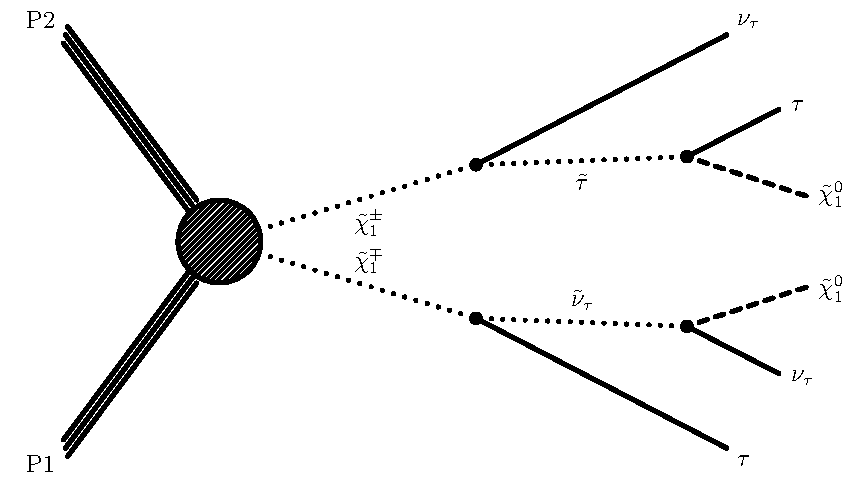
\includegraphics[width=0.49\textwidth]{Introductionfigs/TChipmSlepSnu.pdf}
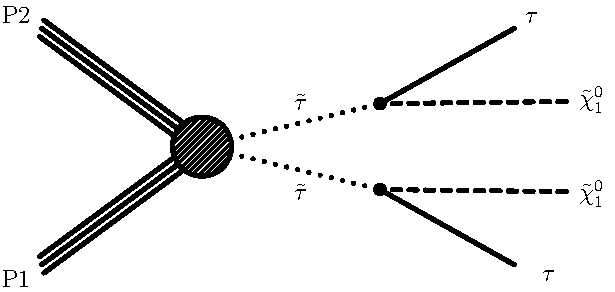
\includegraphics[width=0.49\textwidth]{Introductionfigs/TSlepSlep.pdf}
\caption{Schematic production of double $\tau$ from chargino pair and stau pair.}
\label{fig:Productions}
\end{figure}
%The production cross section of $\PSGcpDo\PSGcmDo$ is more than one order of magnitude higher than the
%production cross section of \sTau\sTau in the same mass of \sTau and \PSGcpDo.  
%For example for a 150 \GeV \sTau or \PSGcpDo, the cross section 
%of the pair production is 27 $fb$ and 1170 $fb$, respectively. Due to the higher cross section, 

Throughout this paper we focus on $\PSGcpDo\PSGcmDo$ production, where \sTau and $\sNu_{\tau}$ 
are produced  on-shell and their masses are the mean value of the masses of the \chione and \PSGczDo.
The \chione decays exclusively via the shown diagram and no other leptons contribute.
%The two distinct decay chains in the left diagram of Fig.~\ref{fig:Productions} are assumed to have equal branching ratios, which is 50\%.

Although the search is sensitive to any 
new physics process with taus and \MET, an R-parity conserving Simplified SUSY Model \cite{Alwall:2008ag,alves:sms} is used 
%to illustrate the performance of the method.
in the end to interpret the results.
Searches for SUSY in di-$\tau$ final state have also been reported by the ATLAS collaboration \cite{Aad:2014yka}. Their search has ruled out 
chargino masses up to 345 \GeV for a massless \PSGczDo, in the similar production diagram.

%In the context of MSSM, supersymmetric objects are produced in pairs to conserve R-parity quantum number. Therefore in the production of charginos from proton-proton collisions, one may consider the following interaction $$pp\rightarrow\PSGcpDo\PSGcmDo\rightarrow\sTau^{+}\nu_\tau \sTau^{-}\nu_\tau\rightarrow\tau^{+}\PSGczDo\nu_\tau\tau^{-}\PSGczDo\nu_\tau\rightarrow\tau^{+}\tau^{-} + 2\,\PSGczDo + 2\,\nu_\tau.$$ In the detector, what can be observed are only 2 tau leptons plus missing transverse energy from the presence of neturinos and neutralinos in the final state.\\ 
%The $\tau$ leptons decay leptonically ($e$ or $\mu$), in 35\% of the time, or decay via hadrons, which occurs in 65\% of the cases. Since there are two $\tau$ leptons in the final state, the probability of having $\PSGcpDo\PSGcmDo \rightarrow \hadtau+e/\mu+\MET$ is about 46\%, while the probability for $\PSGcpDo\PSGcmDo \rightarrow \hadtau+\hadtau+\MET$ to occur is about 42\%. Hereafter, final states containing a lepton are referred to as $\leptonTau$ channel and those events where the two $\tau$'s decay via hadrons are referred to as $\tauTau$ channel. 
%The selection cuts to enhance $\tauTau$ events will be discussed in Section~\ref{sect:tauTauCuts}. The list of cuts to select $\leptonTau$ events can be found in Section~\ref{sect:leptonTauCuts}.\\     

The results discussed here are based on a dataset of proton-proton 
collisions at $\sqrt{s}$=8 \TeV
collected with the CMS detector at the Large Hadron Collider (LHC) during 2012, corresponding to integrated
luminosities of 18.1 and 19.6 \invfb in different channels. 
%{\bf (Need to make this consistent with the abstract).}
Our search makes use of the stransverse mass variable (\mttwo), 
which is the natural extension of transverse mass (\mt) to the case 
where two massive particles with equal mass are created in pairs and decay 
%via a chain of jets and leptons 
to two invisible particles accompanied by jets and/or leptons.  We consider final states where
both taus decay hadronically ($\hadtau \hadtau$), or where one tau decays hadronically and the
other one into an electron or muon ($\leptonTau$).
%In the case of R-parity conserving SUSY, the Lightest Supersymmetric Particle (LSP), \PSGczDo in our scenario, 
%escapes  detection and appears as \MET.

The paper is organized as follows.  The CMS detector, the event reconstruction, and the data sets are described
in Section \ref{sect:CMSRec}; the \mttwo variable is introduced in Section \ref{sect:mt2def}; 
the event selections for the two channels ($\hadtau \hadtau$ and $\leptonTau$)
are described in Sections \ref{sect:tauTauCuts} and \ref{sect:eleTauCuts}, respectively;
a detailed study of the SM backgrounds is presented in Section \ref{sect:bkg}, while Section \ref{sect:sys} 
is devoted to the evaluation of the systematic uncertainties.  The result of the search with its statistical interpretation is presented in 
Section \ref{sect:stat}, and the paper is finally summarized in Section \ref{sect:conclusion}.





